\documentclass[twocolumn]{article}
\usepackage{graphicx}
\usepackage[utf8]{inputenc}
\usepackage[a4paper, margin=0.79in]{geometry}
\usepackage{lastpage}
\usepackage[compact]{titlesec}

\titleformat{\section}[hang]{\bfseries\large}{\thesection}{0.5em}{}
\titleformat{\subsection}[hang]{\bfseries\normalsize}{\thesubsection}{0.5em}{}
\titleformat{\subsubsection}[runin]{\bfseries\normalsize}{\thesubsubsection}{0.5em}{}

\title{\large{\textbf{Systme Validation - Wafer Control}}}
\author{
    \small Ester Vicario ()
    \and \small Gerardo Moyers (4820800 , gmoyersbarrera)
    \and \small Teresa ()
      \and \small yuri ()
}
\date{}

\begin{document}

\maketitle

\begin{center}
    \footnotesize{Report contains \pageref{LastPage} of maximum 6 pages.}
\end{center}

\section{Introduction}
The System Validation course IN4387 is going to be dedicated to find the most efficient solution and validation of the production of silicon wafers. The goal of this assignment is to optimize and evaluate the preparation of the wafers using a control system. By evaluating the process in mcrl2 software it can be determined the feasibility of the implementation. 



\section{Requirements of the system}
During this part of the project and with the main objective of simplify the aspects of it, four components are gonna be considered: 1)the light, 2) both robots R1 and R2, 3) both air lockers with their respective output and input doors and 4) the robot R3.
The requirements of each component will be enumerate a continuation 


\begin{itemize}
\item Light requirements
\begin{itemize}
\item{The light should project the design  when there is a wafer in case there is no wafer it should remain switched off.}
\end{itemize}
\item Air lockers

\begin{itemize}
\item{Both output and input doors can not be open at the same time.}
\item{The  DOi doors should open when they detect that there is something at the input or that a wafer is ready to go to the output.}
\item{The input DIi doors should behave  opening when a wafer is ready to be designed in the lamp or is ready to be delivered to the output. }
\item{Doors should detect if there is any object that needs to enter in the air locker or leave it}

\end{itemize}
\item Robots R1 and R2
\begin{itemize}
\item {Robots must decide if taking an object of dropping in the input or output stacks depending on the airlockers availability an capacity of the stacks}
\item {Once noticed a wafer is  ready in the inputs robots should detect if the airlock is empty}
\item{A robot will have to check if the output stack is full before dropping a wafer}

\end{itemize}
\item Robot R3
\begin{itemize}
\item {Robot R3 will only move when the input doors are opening.}
\item {Robot R3 will not move to the light until the processing of the wafer has finished}
\end{itemize}
\end{itemize}


%Briefly describe the systems you have benchmarked on, and by which methods you have measured.

\section{Interactions and Architecture}
\subsection{Interactions}
The system has 4 elements that can have interactions; Robots R1, R2, Stack, Airlock, light and Robot R3.
\begin{itemize}
\item Robots R1, R2


The main function of the robots R1 and R2 is to pick up or drop the wafer in the input and/or output stacks and transport the wafer between the stacks and the airlock doors.
In this case with the main objective of simplify the process both robots are going to be modeled with the same characteristics and requirements and they are not going to interact between them.  R1 will only be in contact with the input and output stacks 1 and the A1 .
The robot 2 , therefore, will be interacting with the door and stacks 2.


With respect to the wafer stacks the interactions that the robot will have with the stacks with the use of sensors are the following ones
\begin{itemize}
\item{ need to go to the input stack and pick a wafer} 
\item{need to go to the output stack and drop a wafer}
\item{ask for stack status periodically and check if they are full or empty}
\end{itemize}

With respect to the transfer of the wafer from/to the airlock the robots should do the following interactions internally and with the airlock sensors
\begin{itemize}
\item{go to airlock if the door is opening and a wafer should be pick to drop in the output stack }
\item{request door open: a wafer is needed to deliver to the airlock }
\item{check door status periodically: open and/or close}
\end{itemize}

\item Stack


The stack only has to communicate with the robots R1 and R2. The communication will consist in checking the status of the stack and sending the robot where it can put or take a wafer.
\begin{itemize}
\item{ send status (Take me or Go away) }
\end{itemize}
\item Airlock
The airlock interactions is complex, that's because it communicates with the robots outside and the inside robot too. Also it have the restriction that inside door (Din) and outside door (Dout) can't be open at the same time, so it has to keep track of the doors status. 
The interaction between the robot and the airlocks is a communication regarding the status of the doors. At first it receives a request from robots to open the door, when it is open it will send the status of the door and the airlock to the robot so the robot can take or put a wafer.  
\begin{itemize}
\item{ request open door received, proceed to open door}
\item{ check door status to prevent any problem and confirm it is completely open}
\item{ send door status (open/close) and airlock status (wafer/not wafer) }
\item{ close the door}
\item{check if wafer present}

\end{itemize}

\item Robot R3
The main function of robot R3 is to pick the wafer from the airlock and take it to the light, once the light is ready deliver back to the airlock. Therefore, robot R3 should interact with the light and both airlocks whose following interactions are described below:
\begin{itemize}
\item{Pick/place wafer in the airlock. }
\item{Request door open when a wafer has already been processed in the light.}
\item{Check lamp status, if it is ready place a wafer on it, once finish, return the wafer to the airlock available}
\item{ Check door status and airlock status, if door is open and airlock empty a wafer can be placed if the airlock is working R3 wait and checks the status of the other airlock.}
\end{itemize}
\end{itemize}

\begin{itemize}
 
\item Light 

The light should mainly interact with itself as it has to sense if there is a wafer inside and send an end of processing signal .

\begin{itemize}
 \item check if  a wafer is  present
\item lamp light turn on or off
\item check for error
\item send status  to teh robot R3 
\end{itemize}

\end{itemize}
\subsection{Architecture}

The complete scheme of the interactions between the different controllers is depicted in the following picture:
\begin{figure}[t]
    \centering
    \includegraphics[width=\textwidth]{Block_diagram.pdf}
    \caption{Complete system block interactions.}
    \label{fig:complete}
\end{figure}

The lamp system is described in the picture \ref{fig:Lamp_architecture}
\begin{figure}[t]
    \centering
    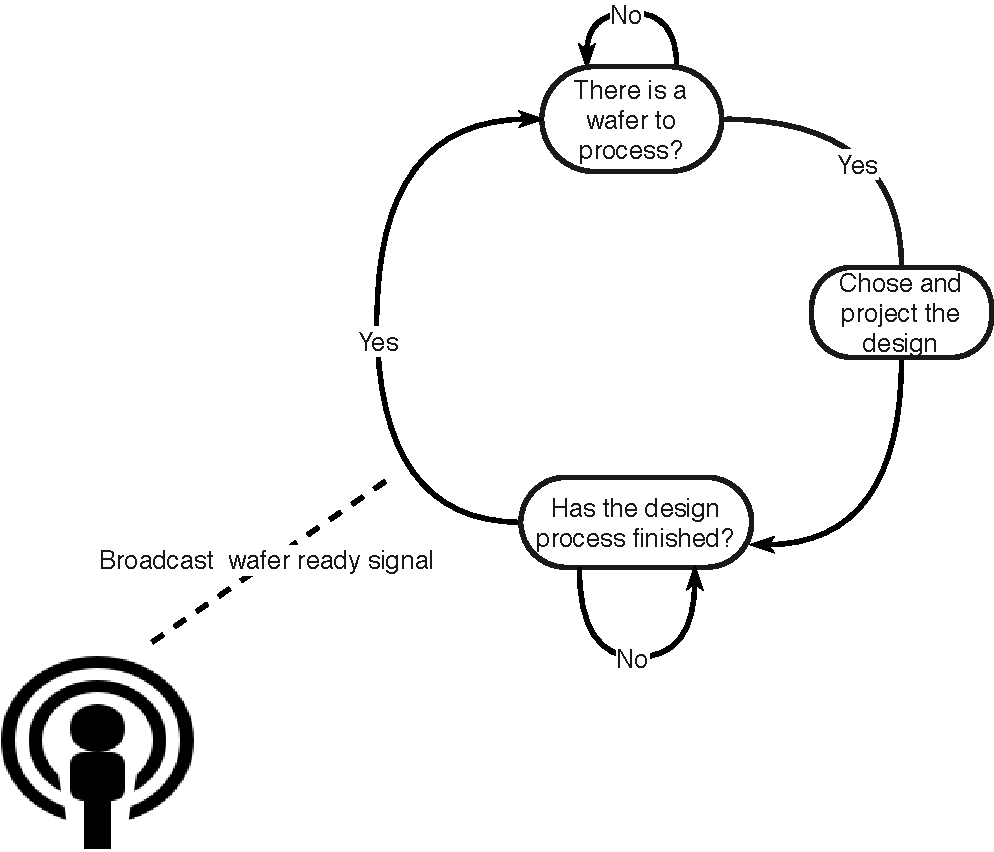
\includegraphics[width=0.45\textwidth]{lamp.pdf}
    \caption{Lamp architecture}
    \label{fig:Lamp_architecture}
\end{figure}


\end{document}
